%INTRO
La scelta del modello di machine learning da utilizzare è in gran parte determinata dalle caratteristiche dei dati a disposizione.

Iniziamo dunque con un analisi del nostro dataset per individuare le caratteristiche che descrivono gli attributi e in che modo i valori che assumono sono distribuiti nelle nostre istanze.

\section{Analisi esplorativa}

Il dataset integrato risultante possiede per ciascuno dei 128 000 tiri informazioni relative al tiro e dati relativi agli atleti coinvolti nello scontro che ha portato allo stesso.
\par

In Shot logs sono stati esclusi alcuni attributi (descritti nella \autoref{tabella_shot_logs}) riguardanti la partita come \texttt{W}, \texttt{Final margin} e \texttt{Matchup}, ritenuti non rilevanti per le sorti di un tiro a canestro.
Anche \texttt{Period} e \texttt{Game clock} sono stati ritenuti superflui, in quanto è già presente l'attributo \texttt{Shot number}, così come non significativo è stato valutato l'attributo \texttt{Pts type} (deducibile dall'attributo \texttt{Shot distance}). 
\par
Analogamente, in Seasons stats sono state escluse decine di indici statistici non determinanti, oltre agli attributi (descritti in \autoref{tabella_seasons_stats}) come \texttt{Games} e \texttt{MP}.

\par
Nell'analisi di questi dati, è emerso lampante che avere a disposizione altri fattori più circostanziali al tiro, che sono reperibili grazie al \textit{visual tracking}, come la parabola del tiro stesso, la velocità dell'attaccante e del difensore, le coordinate sul rettangolo di gioco dei due giocatori e così via, avrebbe aiutato a creare modelli più approfonditi in modo da fornire predizioni più fedeli.
Riprendiamo la possibilità di usare altri dati nella \autoref{metrichemancanti}.

\begin{figure}[H]
\caption{Distribuzione degli esiti nel dataset integrato}
\label{dist_shot_result}
	\includegraphics[scale=0.5]{shot_result}
\end{figure}

I valori da predire sono distribuiti in modo non uniforme. Il 55\% (70 157 record) sono tiri \textit{missed}, mentre il 45\% (57 900 record) sono tiri \textit{made}(\autoref{dist_shot_result}).

\begin{figure}[H]
\centering
\caption{Importanza delle feature, secondo il modello prodotto}
\label{importance_fig}
	\includegraphics[scale=0.9]{importance-svm-25k}
\end{figure}

\par

\textit{Importance}, mostrata nella \autoref{importance_fig}, rappresenta il contributo informativo delle feature considerate. Le principali risultano \texttt{shot\_dist}, \texttt{close\_def\_distance} e \texttt{dribbles}.

\begin{figure}[H]
\caption{Correlazione tra gli attributi più rilevanti}
\label{plot_shot_dist_def}
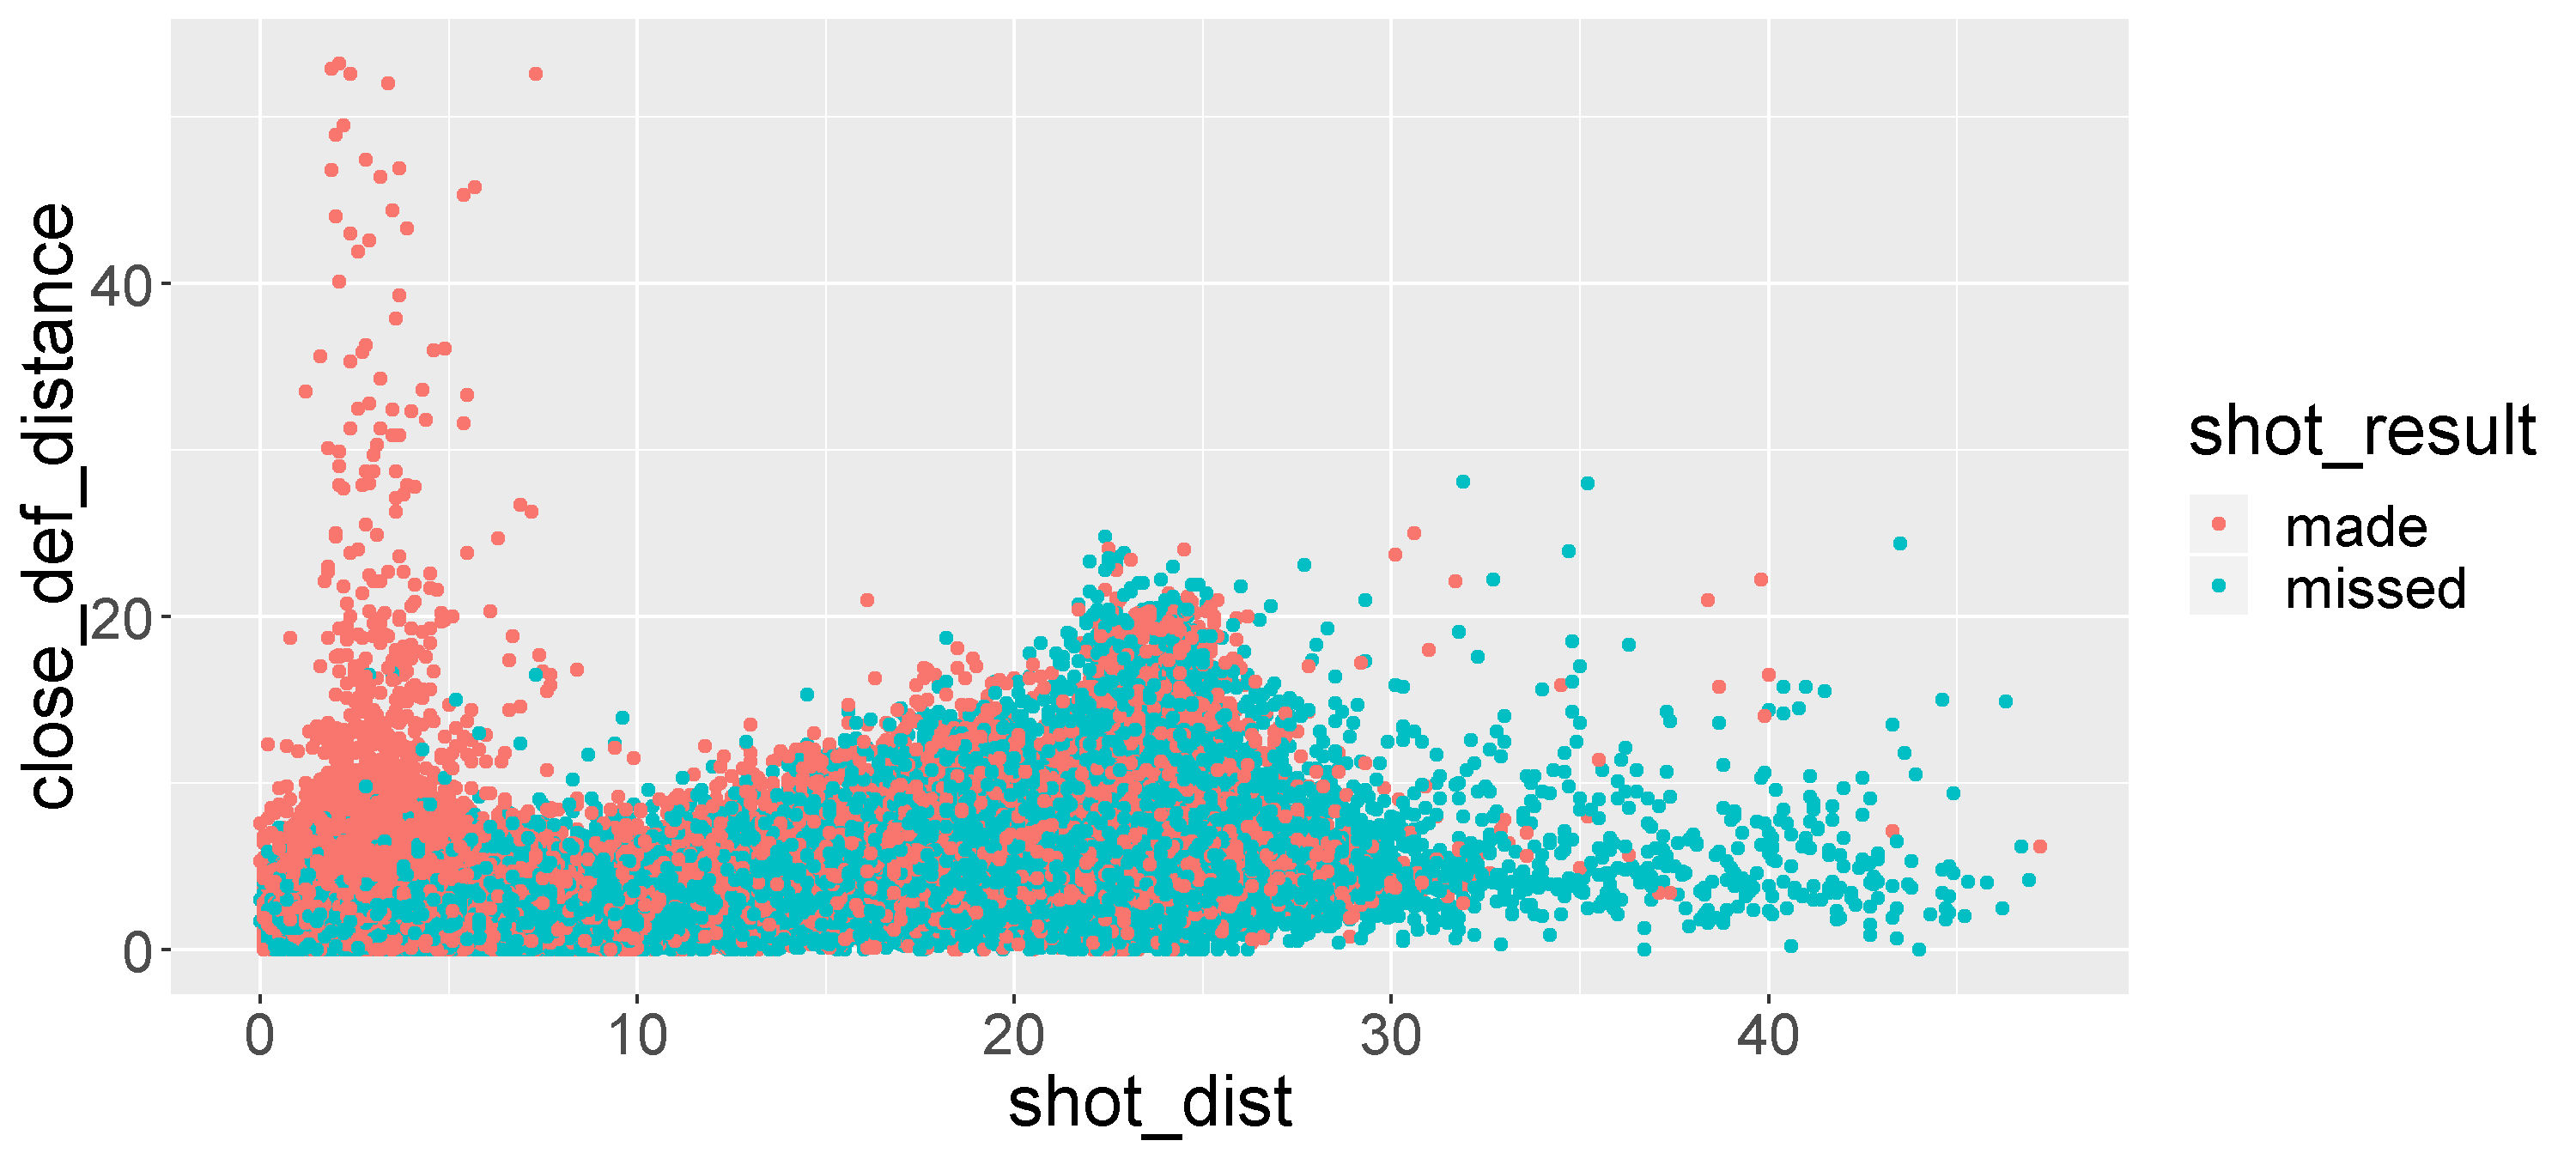
\includegraphics[width=\linewidth]{plot_shot_dist_def.png}
\end{figure}

Il grafico in \autoref{plot_shot_dist_def} è stato interpretato considerando due regioni: la regione con prevalenza \texttt{made}, ossia quella compresa tra $[0, 10]$ nell'asse delle ascisse e $[5, 60] $ nell'asse delle ordinate, e la regione con prevalenza \texttt{missed}, ossia quella compresa tra $[25, 40]$ nell'asse delle ascisse e $[0, 20] $ nell'asse delle ordinate.
Abbiamo intepretato le distribuzioni di queste due regioni rintracciando quello che succede sul campo: i tiri effettuati dal pitturato (area sottostante al canestro), seppur con il difensore molto vicino, hanno una probabilità di essere messi a segno molto alta. I tiri effettuati dalla distanza, invece, sono notoriamente più difficili ed in questo caso è la probabilità di fallimento ad essere più elevata.

\par

\begin{figure}
\caption{Distanza media del tiro rispetto al ruolo del giocatore}
\label{position_shot_dist}
\includegraphics[width=\linewidth]{shot_dist_with_position}
\end{figure}

Il grafico in \autoref{position_shot_dist} mostra che C, il componente della squadra che domina il pitturato, tira in media da una distanza inferiore ai 10 piedi, seguito da PF. I giocatori in questo ruolo prendono quindi tiri ad indice di difficoltà più basso rispetto alla media.
Non abbiamo a disposizione informazioni relative a peso e altezza, ma i dati \cite{basketball-reference} mostrano che in media in questi due ruoli giocano gli atleti più fisicamente dotati: soffrendo meno il contatto con l'avversario riescono a raggiungere più facilmente il canestro.

Al contrario, gli altri tre ruoli (PG, SF e SF) tirano da una distanza che si aggira intorno ai 15 piedi. Solitamente sono meno prestanti dal punto di vista fisico ma con un'abilità al tiro superiore, che li porta a prendere anche tiri di notevole difficoltà dalla distanza.

\begin{figure}[H]
\caption{Successo dei tiri rispetto al ruolo del giocatore}
\label{position_shots}
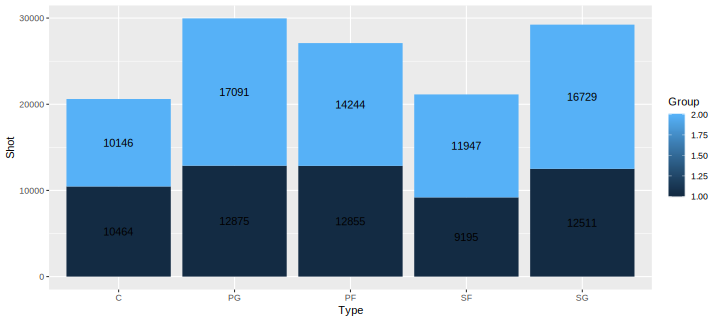
\includegraphics[width=\linewidth]{made_missed_barplot}
\end{figure}

La \autoref{position_shots} conferma questa intepretazione: PF ha una percentuale di missed pari a 0.53, mentre addirittura inferiore (0.49) è la la percentuale di missed per C, per di più l'unico ruolo ad avere un numero di tiri made maggiori rispetto ai missed ma anche quello con il minor numero di tiri effettuati.
Gli altri tre ruoli (PG, SF, SG) hanno una percentuale di missed pari a 0.57.

\pagebreak

\section{Scelta del modello}
% Scelta di C (complexity paramater) e Sigma (gaussian kernel parameter)

Il nostro dataset integrato ha un buon numero di attributi, sia numerici che categorici.
Abbiamo quindi deciso di utilizzare SVM, un algoritmo di apprendimento automatico supervisionato ampiamente utilizzato per problemi di classificazione. Il suo punto di forza è l'utilizzo del cosiddetto \textit{kernel trick}, strumento matematico per mappare l'input in uno spazio multi-dimensionale. SVM performa bene con dataset composti da tanti attributi e numerose osservazioni, adeguato sotto questo punto di vista al nostro caso.
La presenza di attributi categorici porterebbe a preferire gli alberi di decisione, ma esistono alcune tecniche che possono trasformare queste tipologie di campi affinchè siano compatibili anche con le SVM.
